\documentclass[11pt]{article}
\usepackage[utf8]{inputenc}
\usepackage[english, german]{babel}
\renewcommand{\baselinestretch}{1.05}
\usepackage{amsmath,amsthm,verbatim,amssymb,amsfonts,amscd, graphicx}
\usepackage[]{mathtools}
\topmargin0.0cm
\headheight0.0cm
\headsep0.0cm
\oddsidemargin0.0cm
\textheight23.0cm
\textwidth16.5cm
\footskip1.0cm
\setlength\parindent{0pt}
\theoremstyle{plain}
\newtheorem*{theorem}{Theorem}
\newtheorem*{beispiel}{Beispiel}
\newtheorem*{lemma}{Lemma}
\newtheorem*{satz}{Satz}
\newtheorem*{definition}{Definition}
\renewcommand*{\proofname}{Beweis}
\newcommand{\R}{\mathbb{R}}
\newcommand{\Q}{\mathbb{Q}}
\newcommand{\C}{\mathbb{C}}
\newcommand{\N}{\mathbb{N}}
\renewcommand{\i}{\mathrm{i}}
\newcommand{\e}{\mathrm{e}}
\newcommand{\norm}[1]{\left\Vert #1 \right\Vert}
\newcommand{\abs}[1]{\left| #1 \right|}
\newcommand{\diam}{\mathrm{diam}}
\newcommand{\dd}[2]{\frac{d{#1}}{d{#2}}}
\newcommand{\pd}[2]{\frac{\partial #1 }{\partial #2}}
\newcommand{\trace}{\operatorname{tr}}
\newcommand{\oo}{\infty}
\newcommand{\sign}{\operatorname{sign}}
\newcommand{\Forall}{\quad\forall\,}
\renewcommand{\d}[1]{\,d#1\,}
\usepackage{braket}
\usepackage{centernot}
\usepackage{tikz}
\usetikzlibrary{matrix}

% \renewcommand{\labelitemi}{$\blacktriangleright$}
% \renewcommand{\labelitemii}{$\vartriangleright$}
% \renewcommand{\labelitemiii}{$\bowtie$}
% \renewcommand{\labelitemiv}{$\star$}
\newcommand{\sumint}{\ooalign{$\textstyle\sum$\cr\hidewidth$\displaystyle\int$\hidewidth\cr}}

\usepackage{enumerate}
\usepackage[pdf]{pstricks}
\usepackage{epsfig}
\usepackage{pst-grad} % For gradients
\usepackage{pst-plot} % For axes
\usepackage{siunitx}
\usepackage{varwidth}
\newenvironment{centerall}
{\begin{center}\begin{varwidth}{\textwidth}}
{\end{varwidth}\end{center}}

% \usepackage{MnSymbol}
\begin{document}
\section{Einf\"uhrung}
\emph{Schwabl Kapitel 1.1} \\
\begin{description}
  \item Makroskopische Systeme aus $N \gg 1$ Teilchen.
  \item Mikrozustand und mikroskopische Gesetze
    \begin{itemize}
      \item Klassische Physik: 
        \[\text{Punkt } (\vec{r}, \vec{p}) \in \text{ Phasenraum} \simeq \R^{6N} \]
        \[ m_1 \ddot{\vec{r}} = \vec{F}_1 \]
      \item Quantenmechanik: 
        \[ \text{Wellenfunktion } \Psi (\vec{r},t) \in \mathcal {L}_2 (\R^{3N}) \]
        \[ i \hbar \pd{\Psi}{t}= H \Psi \]. 
    \end{itemize}
    
  \item Makrozustand und Makroskopische Gesetze
    \begin{itemize}
      \item Temperatur $T$, Volumen $V$, Druck $P$, ...
      \item $P V=nk_BT, \quad U=RI$
    \end{itemize}
  \item Mikroskopische Gesetze $\implies $ makroskopische Gesetze.
  \item Makrozustand $\iff $ Zeitmittelung
    \begin{itemize}
      \item Klassische Physik: \[ \bar{A}(t)= \frac{1}{\Delta t} \int_{t}^{\Delta t +t}
        dt'\, A(\vec{r}(t'),\vec{p}(t'))\] 
      \item Quantenmechanik: \[ \bar{B}(t) = \frac{1}{\Delta t} \int_{t}^{\Delta t+t}
        dt' \Braket{\Psi(t) | \hat{B} | \Psi (t)}\] 
    \end{itemize}
  \item Mikroskopische Zeitskala $\ll\, \Delta t \, \ll$ makroskopische Zeitskala
  \item Statistische Mittelung
    \begin{itemize}
      \item Klassische Physik \[ \bar{A} = \int_{}^{} d^3r\, d^3p\,
        A(\vec{r}, \vec{p}) P(\vec{r}, \vec{p}), \quad
        \text{ Wahrscheinlichkeitsdichte } P(\vec{r}, \vec{p}) \] 
      \item Quantenmechanik: \[ \bar{B}= \trace(\hat{B} \hat{\rho})
          \text{ Dichteoperator } \hat{\rho} \]   
    \end{itemize}
  \item Statistische Physik
    \begin{itemize}
      \item Bestimmung von $P$ und $\hat{\rho}$
      \item Berechnung der Ensemblemittelung
      \item Anwendung auf physikalische Probleme
    \end{itemize}
  \item Reduktionismus \[ \text{System } = \left\{ \text{Einzelteile} \right\} \] 
    %TODO: make this a flow diagram
  \item Elementarteilchenphysik $\to $ Festk\"orperphysik, Chemie $\to $
    Biologie $\to $ Medizin $\to $ Psychologie $\to $ Soziologie
  \item ``\emph{More is different}'' P.W. Anderson
    %TODO: add pictures of snowflakes
    
\end{description}
\section{Wahrscheinlichkeitstheorie}
\emph{Schwabl Kapitel 1.2, 1.5.1} \\
\begin{description}
  \item [Einige Definitionen]

  \item [Zufallsvariable $x$] Wert von $x$ h\"angt von einem Zufallsereignis ab
    Beispiel Messung: $x= X_{\text{exakt}} + \text{ Messfehler }$

  \item[H\"aufigkeit] 
    $N$ identische Versuche, $N_x = \text{ Anzahl der Werte } x \implies \frac{N_x}{N}$

  \item[Empirische Wahrscheinlichkeit]
    $P_x = \lim\limits_{N \to \infty } \frac{N_x}{N}$.
    \[ \sum_{x}{} P_x = 1 , \quad 1 \ge P_x \ge 0 \quad \] 

  \item[Wahrscheinlichkeitsdichte] 
    $w(x) \quad x \in \R$. \[ w(x)\Delta x = \text{ Wahrscheinlichkeit f\"ur einen
      Wert } \in [x, x+\Delta x]  \] 
      \[ \int_{}^{}dx\, w(x)=1, \quad w(x)\ge 0 \] 
      Beziehung mit diskreter Warscheinlichkeit: 
      \[ w(x) = \sum_{i}{}P_i \delta ( x-x_i) \] 

  \item[Mittelwert/Erwartungswert]
    \[ \Braket{f(x)} = \sum_{x}{} f(x) P_x \text{ beziehungsweise } \int_{}^{}
      dx\, w(x) f(x)\] 

  \item [Schwankungsquadrat] \[ \Delta X^2 = \Braket{(x-\Braket{X})^2}
    = \Braket{X^2}- \Braket{X}^2 \quad \Delta x \Delta p \ge \hbar/2\] 
\end{description}
\subsection{Zentraler Grenzwertsatz}
Es gibt $N$ unabh\"angige aber identische Zufallsvariablen $x_i, \, i=1 , \dotsc , N$.
\[ P(x_1,\dotsc,x_N)= P(x_1) P(x_2) \ldots P(x_N)  \]
Au\ss{}erdem existieren $\Braket{x},\Delta x$ von  $P(x)$.
\[ \text{Mittelwert } Y= \frac{1}{N}\sum_{i=1}^{N}x_i  \text{ ist eine
Zufallsvariable mit Wahrscheinlichkeit } Q_N(Y) \] 
\[ Q_N(Y) \xrightarrow{N\to \infty}\frac{1}{\sqrt{2 \pi} \sigma}
\exp{(-\frac{(Y-a)^2}{2 \sigma^2})}\] 
\[ a=\Braket{x}, \quad \sigma= \frac{\Delta x}{ \sqrt{N}} \] 


\begin{figure}[htpb]
  \centering
  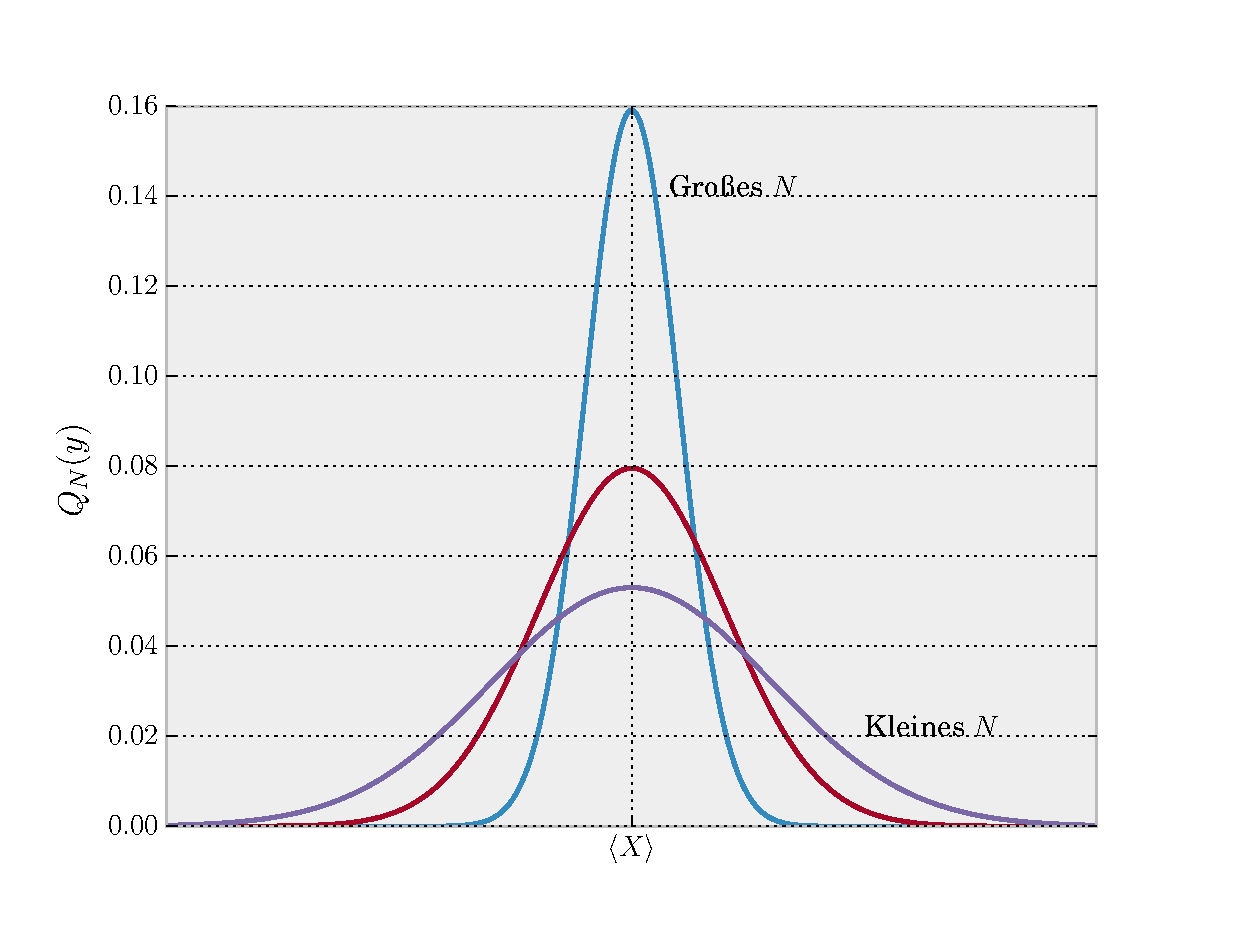
\includegraphics[width=0.8\textwidth]{./figures/first.eps}
  \caption{Normalverteilung, $Y=\Braket{X} \pm \frac{\Delta X}{\sqrt{N}} $}
  \label{fig:first}
\end{figure}
\section{Klassische Physik}
\begin{description}
  \item[N Teilchen ] Mikrozustand $(q,P) \in  \text{ Phasenraum } \simeq \R^{6n}$
  \item[Kanonische Gleichungen] \[ \dot{q}_j = \pd{H}{P_j} \quad \dot{P}_j = \pd{H}
    {\dot{q}_j}, \quad j=1,...,3N \] 
  \item[Anfangsbedingung] \[ (q_0, P_0)= (q_0(t_0), P(t_0)) \implies \text{ Bahn }
    (q(t | q_0, P_0), P(t| q_0, P_0)) \] 
  \item[Kanonische Transformation ] \[ (q(t), P(t)) \iff (q(t'), P(t')) \] 
  \item[Ziel] \[ \bar{A}= \int_{}^{} d^{3N}q\, d^{3N}p\, A(q,P) P_G(q,P) \] 
    Gleichgewichtsverteilung $P_G(q,P)= $?
  \item[Unscharfe Angangsbedingung] \[ P(q,P,t_0)= P_0 (q,P) \] 
    Scharfe Anfangsbedingung: $P_0(q,P) = \delta(q-q_0) \delta (P-P_0)$.
    Differentialgleichung f\"ur $P(q,P,t)$: Liouville-Gleichung.
    \[ P(t)= P(q,P,t)\, d^{3N}q\, d^{3N}p=P(t') = P(q,P,t')\, d^{3N}q'\, d^{3N}p' \] 
  \item[Liouville-Satz] \[ d^{3N}q\, d^{3N}p = d^{3N}q'\, d^{3N}p' \quad \left[
    \text{ Jacobi-Matrix } \frac{d^{3N}q'\, d^{3N}p'}{d^{3N}q\, d^{3N}p}= 1 \right] \] 
    \[ \implies P(q(t), P(t), t)= P(q(t'), P(t'), t'), \quad
    \text{ Erhalungsgr\"o\ss{}e } \frac{dP}{dt}=0 \] 
  \item[Kettenregel] \[ \frac{d P(q(t), P(t),t)}{dt}= \pd{P}{t} + \left\{ H,P \right\} \] 
  \item[Liouville-Gleichung] \[ \pd{P}{t}= \left\{ P,H \right\} \] 
    Bedingungen f\"ur $P_G(q,P)$ (im Gleichgewicht)
    \begin{itemize}
      \item $\left\{ P_G, H \right\}=0$
      \item $P_G \ge 0$
      \item $\int_{}^{}d^{3N}q\, d^{3N}p\, P_G (q,P)=1$.
    \end{itemize}
    Superpositionsprinzip: L\"osungen $P_1,P_2 \implies P=a_1 P_1+ a_2 P_2 $
    mit $a_1,a_2 \ge 0, \quad a_1+a_2 =1$. \\
    Makrozustand: $T,V,P,... \quad  \implies P_0 \text{ oder } P_g$?\\
\end{description}
\section{Quantenmechanik}

\emph{Schwabl Kapitel 1.4,1.5.2}\\
$N $ Teilchen, Mikrozustand $\Ket{\Psi} \in \mathcal{H} \simeq \mathcal{L}_2(\R^{3N})$
\begin{align*}
  i \hbar \frac{d}{dt} \Ket{\Psi(t)} = H \Ket{\Psi(t)} \\
  \text{Anfangsbedingung } \Ket{\Psi_0} \to \Ket{\Psi(t)} \quad \text{(eindeutig)} \\
  \text{Erwartungswert } A(t)= \Braket{\Psi(t) | \hat{A} | \Psi(t)} =\Braket{\hat{A}}\\
\end{align*}
Ziel: \[ \text{Statistische Mittelung } \quad \Braket{\hat{A}} = \trace(\hat{A}\hat{\rho}_G), \quad \hat{\rho}_G=? \] 
\subsubsection*{Definition}
Statistischer Operator, Dichteoperator, Dichtematrix, ...
\begin{align*}
  \hat{\rho} & : \mathcal{H} \to  \mathcal{H}, \text{ linear } \\
  \hat{\rho} & = \hat{\rho}^+\dagger \\
  \text{positiv-semidefinit } & \Braket{\varphi | \hat{\rho}| \varphi} \ge 0 \,\forall\,\Ket{\varphi} \in \mathcal{ H} \\
  \trace \hat{\rho } & =1  &
  \text{Spektrale Zerlegung } & \begin{split}
  \hat{\rho} &=  \sum_{n}^{} p_n \Ket{n}\Bra{n} \\ &= \int_{}^{} d \lambda \Ket{\lambda}\Bra{\lambda} w(\lambda) 
  \end{split}
   \\
  \text{Dichteoperator } & \implies \begin{matrix} p_n \ge 0 \\ \sum_{n}^{} p_n =1 \\
p_n \in \R \end{matrix} 
&
\begin{matrix} 
  w(\lambda )\ge 0 \\ \int_{}^{} d \lambda w( \lambda )=1 \\ w(\lambda) \in \R 
\end{matrix} \\
  \Braket{\hat{A}}= \sum_{n}^{}p_n \Braket{n|\hat{A}|n}.
\end{align*}
\begin{description}
  \item[Reiner Zustand]: \[ p_{n_0}=1,\, p_n =0 \,\forall\, n \neq n_0, \quad  \hat{\rho}= \Ket{n_0}\Bra{n_0} \implies \hat{\rho}^2=\hat{\rho} \]  
  \item[Gemisch]: $p_n \neq 0 $ f\"ur 2 oder mehr $n$.
    \begin{itemize}
      \item Verschr\"ankte Zust\"ande
      \item Statistisches Gemisch
    \end{itemize}
  \item[Spektrale Zerlegung] \begin{align*}
    \hat{A} &= \sum_{\alpha}^{}a_ \alpha \Ket{\alpha}\Bra{\alpha} \\
    \Braket{A}&= \sum_{n}^{}p_n \sum_{\alpha}^{}a_ \alpha \abs{\Braket{n|\alpha}}^2
    = \sum_{n}^{}\sum_{\alpha}^{} \underset{\text{Stat. Zufall}}{p_n} \underset{\text{Q.M. Zufall}}{\abs{\Braket{n|\alpha}}^2} a_ \alpha
  \end{align*}
  % TODO: Fig 4
  \[ \text{Gemisch: 2 Quellen: } I_1, \theta_1, \quad I_2, \theta_2 \implies 
  I'= I_1 ( \cos{\theta_1})^2 + I_2 (\cos{\theta_2})^2 \] 
  \[ p_1 = \frac{I_1}{I_1 + I_2}, \quad p_2 = \frac{I_2}{I_1 + I_2} \] 
\end{description}
\subsection*{Von Neumann Gleichung}
\[ i \hbar \frac{d\hat{\rho}}{dt} = \left[ H, \hat{\rho} \right] \] 
\begin{itemize}
  \item Anfangsbedingung $\hat{\rho}_0 \to  \hat{\rho}(t)$
  \item Gleichgewicht: \[ \frac{d \hat{\rho}}{dt}=0 \implies  \left[ H, \hat{\rho} \right]=0  \] 
  \item Superpositionsprinzip $\rho= a_1 \rho_1 + a_2 \rho_2 \text{ mit }
    a_1, a_2 \ge 0, \text{ und } a_1+a_2 =1 $
  \item Im Gleichgewicht: \[ \hat{\rho}_G = \sum_{n}^{} p_n \Ket{E_n}\Bra{E_n}
    = \int_{}^{} dE\, w(E)\Ket{E}\Bra{E} \quad \text{ mit }
    H \Ket{E}= E \Ket{E}\] 
  \item Isoliertes System: \[ p_n = \frac{1}{Z_n} \text{ f\"ur } E_n = E_0,
    \quad Z_n= \text{ Entartung des Niveaus } E_0 \] 
    % TODO: Fig 5
  \item Geschlossenes System: \[ p_n = \frac{1}{Z} e^{-\beta E_n} \text{ mit } 
    \beta= \frac{1}{k_B T}, \quad Z=\sum_{n}^{} e^{-\beta E_n} \] 
\end{itemize}

\subsection*{Entropie und Ensemble}
\emph{Schwabl Kapitel 2.1-2.5}\\
\begin{description}
  \item[Definition] Entropie (Quantenstatistik) \\
    \[ S =-k_B \trace(\hat{\rho} \ln{\hat{\rho}}) \quad k_B = k = 
      \text{ Boltzmann-Konstante }
    \approx \SI{1,38e-23}{\joule\per\kelvin} \] 
  \item[Eigenschaften] 
    \begin{align*}
      \hat{\rho} = \sum_{n}^{} p_n \Ket{n}\Bra{n} && p_n \ge 0 && \sum_{n}^{} p_n = 1 \\
      S(\left\{ p_n \right\}) = -k_B \sum_{n}^{} p_n \ln{p_n}
    \end{align*}
    Hinweise: \begin{align*}
      \trace \hat{A} = \sum_{n}^{} \Braket{n | \hat{A}|n} && f(\hat{\rho})= 
      \sum_{n}^{} f( p_n) \Ket{n}\Bra{n} \\
      e^{\hat{A}}= \sum_{n=0}^{ \oo } \frac{1}{n!}\hat{A}^n
    \end{align*}

    Die Entropie ist also \"uber die Diagonalemente der Dichtematrix in
    diagonalisierter Form berechenbar. Dies ist wohldefiniert, da jede
    Dichtematrix diagonalisiert werden kann.

    Extrema mit Nebenbedingung $\sum_{n}^{} p_n = 1$
    \begin{itemize}
      \item Minimum $S=0$ f\"ur einen reinen Zustand ($p_{n_0}=1, p_n =0
        \quad\forall\, n \neq n_0$)
      \item Maximum $S= k_B \ln{M}$ f\"ur $p_n = \frac{1}{M} \quad\forall\, 1,...,M$.
    \end{itemize}
    Die Entropie ist maximal f\"ur Unkenntnis \"uber den Zustand des Systems
    (Auch ma\ss{} f\"ur Unordnung).
  \item[Extensivit\"at] \[ \mathcal{H}= \mathcal{H}_A \otimes \mathcal{H}_B,
  \quad \hat{\rho} = \hat{\rho}_A \otimes  \hat{\rho}_B \] 
  \begin{align*}
    \hat{\rho}_A \to  \hat{\rho}_A \otimes  \hat{I}_B  \\
    \hat{\rho}_{\hat{B}} \to  \hat{I}_A \otimes  \hat{\rho}_B \\
    \implies \left[ \hat{\rho}_A, \hat{\rho}_B  \right]= 0
  \end{align*}
  \begin{align*}
    S & = -k_B \trace( \hat{\rho} \ln{\hat{\rho}})  \\
      & =  -k_B \trace \left[ (\hat{\rho}_A \otimes \hat{\rho_B}) 
  \ln{(\hat{\rho}_A \otimes \hat{\rho}_B)}  \right]  \\
  & = -k_B \trace (\hat{\rho}_A \ln{ \hat{\rho}_A}) - k_B \trace
    (\hat{\rho}_B \ln{ \hat{\rho}_B}) = S_A + S_B
  \end{align*}
  Nebenbedingung

  \[ S \le S_A + S_B \] (z.B. verschr\"ankte Systeme)
\item[Beispiel] System von $N$ Spins $S$ ($\vec{S}^2 =  S(S+1)$). \\
  Hilbert-Raum f\"ur einen Spin $= \mathcal{H}_1 = \C^{2S+1}$.
  Gesamter Hilbert-Raum \[ \mathcal{H} = \bigotimes_{i=1}^{N} \mathcal{H}_i \] 
  \[ \operatorname{dim} \mathcal{H} = (2S+1)^N = M \] 
  \begin{itemize}
    \item Minimum $S=0$ z.B. f\"ur $\Ket{\Psi} = \Ket{ \uparrow, \uparrow, \uparrow, \ldots, \uparrow}$.
    \item Maximum $S= k_B \ln{M}$ f\"ur $\hat{\rho}= \frac{1}{n} \hat{I}=
      k_B n \ln{(2S+1)}$
  \end{itemize}
\item[Gleichgewicht]
  \begin{align*}
    0= \frac{d \rho }{dt} \iff \left[ H, \hat{\rho} \right]=0 \implies 
    \rho = \sum_{m}^{} p_n \Ket{E_n} \Bra{E_n} \\
    \implies E = \Braket{\hat{H}} = \trace (\hat{\rho} \hat{H})
    = \sum_{n}^{} p_n E_n
  \end{align*}
  \begin{align*}
    \rho \Ket{E_n} = p_n \Ket{E_n} \\
    H \Ket{E_n} = E_n \Ket{E_n}
  \end{align*}
\end{description}
\begin{description}
  \item[Definition]  Statistisches Ensemble oder Gesamtheit \\
    Sie ist eine Gewichtete Menge der Mikrozust\"ande, die einen 
    Makrozustand entsprechen.
    \begin{align*}
      \left\{ ( \Ket{N}, p_n) \right\} \equiv \hat{\rho} = \sum_{n}^{} p_n
      \Ket{n} \Bra{n} 
    \end{align*}
\end{description}
\subsection*{Zentrales Postulat der statistischen Physik}
System mit $N\to \infty$ Freiheitsgraden im Gleichgewicht.
\begin{itemize}
  \item $S$ ist maximal f\"ur einen gegebenen Makrozustand. Das erlaubt uns
    eine eindeutige bestimmung des statistischen Operators $\hat{\rho}$.
  \item Statistische Mittelungen der Observablen erf\"ullen die Makroskopischen
    Gesetze der Thermodynamik.
    %
    \begin{align*}
      S = -k_B \trace \hat{\rho}_B = - k_B \Braket{\ln{\hat{\rho}_G}} \\
    \end{align*}
    %    
    \begin{align*}
      \Braket{\hat{\cal{O}}}= \trace (\hat{\rho}_G \mathcal{O}) &&
      U = \Braket{\hat{H}}
    \end{align*}

\end{itemize}
\begin{description}
  \item[Definition] Entropie (Thermodynamik) \\
    Wir betrachten ein System in einem Bad, mit welchem es Energie austauschen
    kann. Eine ideelle Situation, in welcher alle Prozesse die wir betrachten 
    reversibel sind. 
    \begin{align*}
      dS = \frac{\delta Q}{T}
    \end{align*}
    Zustandsfunktion oder Thermodynaische Variable.
    \begin{itemize}
      \item Extensiv
      \item monoton steigend $\pd{S}{E} > 0$
      \item $ \lim_{T \to 0} \frac{S}{N} = 0$.
    \end{itemize}
\end{description}
\begin{description}
  \item[Nebenbedingung] F\"ur bestimmte Modelle statistische Entropie nicht
    gleich der thermodynamischen Entropie, das bedeutet das Modell ist nicht
    physikalisch. Eigentlich hat man in den letzten 100 Jahren in denen man
    Forschung betreibt kein Problem gefunden, das man nicht l\"osen konnte.
    Es gibt verschiedene Situationen in derr Praxis, in denen man die Makrozust\"ande
    beschreibt. 
\end{description}
\subsection*{Mikrokanonisches Ensemble}
Es beschreibt ein isoliertes System.
\begin{description}
  \item[Freie thermodynamische Variablen] $ $ 
    \begin{itemize}
      \item Teilchenzahl $N$
      \item Volumen $V$
      \item Magnetisierung $M$
      \item Energie $E$
    \end{itemize}
  \item[Zustandsfunktion] Druck $P(N,V,E)$
  \item[Maximierung der Entropie] 
    \begin{align*}
      \hat{\rho} & = \subset P_E P_N \ldots \\
      \hat{\rho} & ~ \delta(\hat{H} - E) \delta (\hat{N} - N)
    \end{align*}
\end{description}
\subsection*{Kanonisches Ensemble}
Beschreibt ein geschlossenes System.
\begin{description}
  \item[Freie thermodynamische Variablen] $ $
    \begin{itemize}
      \item Temperatur $T$
      \item $N, V, M$
    \end{itemize}
  \item[Zustandsfunktionen] $E(T, N, V)$
  \item [Maximum der Entropie] 
    F\"ur feste $T, N, V, \ldots$
    \begin{align*}
      \hat{\rho} = \frac{1}{Z} e^{- \beta \hat{H} } \hat{P}_N \ldots && 
      \beta = \frac{1}{k_B T}
    \end{align*}
  \item[Zustandsumme]
    \begin{align*}
      Z= \trace e^{- \beta \hat{H}}
    \end{align*}
\end{description}

\subsection*{Gro\ss{}kanonisches Ensemble}
Beschreibt ein offenes System
\begin{description}
  \item[Freie Thermodynamische Variablen]  $ $
    \begin{itemize}
      \item Chemisches Potential $\mu$
      \item $T, V, \ldots$
    \end{itemize}
  \item[Zustandsfunktionen] $N(T, \mu, V)$
  \item[Maximum der Entropie] f\"ur feste $T, \mu, V$ falls
    \begin{align*}
      \hat{\rho}_G = \frac{1}{Z_{GK}} e^{-\beta(\hat{H}- \mu \hat{N})} P
    \end{align*}
  \item[Gro\ss{}kanonische Zustandssumme] $Z_{GK} 
    \trace e^{-\beta(\hat{H}- \mu \hat{N})} $
\end{description}
\subsection*{Viele weitere Ensembles}
Zu jeder intensiven Variable gibt es eine Extensive Variable(Observable).

\begin{center}
  \begin{tikzpicture}
    \matrix (m) [matrix of math nodes,column sep=6em,
      column 1/.style={anchor=base east},
      column 2/.style={anchor=base west}
    ] 
    {
      \underset{\text{Intensive Variable}}{\text{\"Au\ss{}eres Feld}} & 
      \underset{\text{Extensive Variable}}{\text{Observable}} \\
      y & x \\
      \hat{\rho}_G ~ e^{- \beta y \hat{x}} & \hat{\rho}_G ~ 
      P_x ~ \delta (\hat{x} -x ) \\
      \text{Beispiele} \\
      M & N \\
      P & V \\
      H & M \\
    \text{Magnetfeld} & \text{Magnetisierung} \\};
  \end{tikzpicture}
\end{center}


 \section*{Mikrokanonisches Ensemble}
 Wir betrachten ein isoliertes System. Zum beispiel ein Gas in einem Beh\"alter
 welcher isoliert ist. Energie und Teilchenzahl sind fest. Genauso das Volumen.
 Eine \"Ahnliche Situation w\"are auch ein magnetisches Material. Die isolation
 w\"are hier ein Material welches keine magnetischen Felder durchl\"asst.
 Typisch f\"ur das isolierte System ist, dass die Energie eine kontrollierbare
 Variable ist.

 Es gibt also eine Freie thermodynamische Variable $E$. Die erlaubten 
 Mikrozust\"ande sind die Eigenzust\"ande des Hamilton-Operators $H$ zur
 Energie $E$.
 Das Ziel ist nun die mikrozust\"ande zu beschreiben und die makroskopischen
 Variablen zu berechnen. Man braucht dazu den statistischen Operator.
 \begin{description}
   \item[Diskretes Eigenspektrum] 
     \begin{align*}
       \hat{\rho} = \sum_{n}^{} p_n \Ket{n}\Bra{n} \quad : \quad \mathcal{H} \to 
       \mathcal{H} && p_n =0 \quad\forall\, n \text{ mit } E_n \neq E \\
       \hat{\rho}= \sum_{n=1}^{w(E)} p_n \Ket{n}\Bra{n} &&
       w(E) = \text{ Entartung der Eigenergie } E
     \end{align*}
     Wir verwenden das Postulat der maximierung der Entropie:
     % \begin{align*}
     %   S(E)= -k_B \sum_{n=1}^{w(E)} p_n \ln{p_n}, && 
     %   \sum_{n=1}^{w(E)} p_n = 1 
     % \end{align*}
     \begin{align*}
       0  &= \pd{S}{p_n} - \lambda \pd{}{p_n} 
       \left( \sum_{n=1}^{w(E)} p_m -1 \right)  \\
       & = -k_B \left( \ln{p_n} +1 \right) - \lambda \Forall 1 ,\dotsc, w(E) \\
     \end{align*}

     \begin{align*}
       \text{ Extrema f\"ur }      
       & \implies p_n = e^{-\frac{\lambda}{k_B} - 1} \implies p_n = \frac{1}{w(E)} \\
       & \implies S(E) = k_B \ln{(w(E))} \text{ ist auch ein Maximum }
     \end{align*}

   \item[Dichteoperator im Gleichgewicht]
     \begin{align*}
       \hat{\rho}_G = \sum_{n=1}^{w(E)} \frac{1}{w(E)} \Ket{n}\Bra{n} =
       \frac{1}{w(E)} P_E = \frac{1}{w(E)} \delta(H-E) & \\
     \end{align*}
     \begin{align*}
       \trace \hat{\rho}_G = 1 && \trace P_E = w(E) \\
     \end{align*}

   \item[Kontinuierliches Spektrum]
     \begin{flalign*}
       \hat{\rho} &= \int_{}^{} d\lambda\, \Ket{\lambda}\Bra{\lambda} p(\lambda) \\
       N(E) &= \text{ Anzahl der Zust\"ande mit einer Eigenenergie } \le E
     \end{flalign*}
     Hinweis: F\"ur ein diskretes System von Eigenzust\"anden
     f\"ur ein kontinuerliches Spektrum kann man die Anzahl der Eigenzust\"ande 
     kleiner Als $w$ definieren.
     \begin{align*}
       w(E) &= \frac{dN}{dE} = \text{ Zustandsdichte } \\ & \implies w(E) \Delta E
       = \text{ Anzahl der Eigenzust\"ande in } \left[ E, E+ \Delta E \right] \\
       S(E) &= k_B \ln{(w(E) \Delta E)} \\
       \hat{\rho} &= \frac{1}{w(E)} \delta(H-E) 
     \end{align*}
 \end{description}
 \subsection*{Thermodynamische Variablen}
 Man macht eine Statistische Mittelung
 \begin{align*}
   \Braket{\hat{\cal{O}}} = \trace (\hat{\rho}_G \hat{\cal{O}})
 \end{align*}
 \begin{description}
   \item[Beispiele] 
     \begin{align*}
      \text{Innere Energie: } U= \Braket{H} = E \\
      \text{Magnetisierung: } M_z = \Braket{S_z} \\
     \end{align*}
   \item[Thermodynamischer Limes] ($N \to \infty$)
   \item[Definition] Temperatur
     \begin{align*}
       \frac{1}{T} = \left( \pd{S}{E} \right)_x
     \end{align*}
   \item[Definition] Konjugierte Variablen \\
     Beispiele: 
     \begin{align*}
       x = \begin{Bmatrix} 
         M \xleftrightarrow{\hspace{1cm}}  H \\ 
         N \xleftrightarrow{\hspace{1cm}}  M \\
         V \xleftrightarrow{\hspace{1cm}} P 
     \end{Bmatrix} y
     \end{align*}
     %
     \begin{align*}
       S(E,X) && y = \pm  T \left( \pd{S}{X} \right)_E
     \end{align*}
     %
   \item[Statistische Physik] $ $ \\
     \begin{align*}
       \text{Extensive Observable } \hat{x}, \quad && [\hat{x}, \hat{H}]
       \xrightarrow{ N \gg 1} N^0, n^{-1} \\
       \implies \Braket{\hat{x}} = x && S(E,X) = k_B \ln{ w(E,X)} \\
     \end{align*}
 \end{description}
\subsection*{Beispiel: System von nicht-wechselwirkenden Spins}
\begin{align*}
  N \text{ Spins } s=1, && H = \sum_{i=1}^{ N } H_i = J \sum_{i=1}^{N} S_{iz}^z
  \quad (J>0) \\
\end{align*}

Eigenzust\"ande: 

\begin{align*}
  \text{1 Teilchen } & \begin{cases}
    H_i \Ket{M_j} = J S_{j z}^z \Ket{m_j} = J \hbar^2 m_j^2 \\
    S_{zj} \Ket{m_j} = \hbar m_j \Ket{m_j} &  m _j = -1,0,1 \\
  \end{cases} \\
  \text{$N$ Teilchen } & \begin{cases}
    \text{Dim } \mathcal{H} = 3^N \\ %REALLY? \\
    \Ket{ \left\{ m_j \right\} }= \Ket{m_j} \otimes \Ket{m_j} \otimes  \ldots 
      \otimes  \Ket{m_N} \\
      E(\left\{ M_j \right\})= J \sum_{j=1}^{N}m_j^2 \\
      S_z \Ket{ \left\{ m_j \right\} }= {\sum_{j}^{} m_j } & M=\sum_{j}^{}
      m_j
      \Ket{ \left\{ m_j \right\} }
  \end{cases} \\
  & H\Ket{ \left\{ m_j \right\} } = E (\left\{ m_j \right\}) \Ket{ \left\{ m_j \right\} }
\end{align*}

\begin{description}
  \item[Problem]  Entartung $w(E,M)$ \\
    \begin{align*}
      N_+ & = \text{ Anzahl der Spins mit } m_j = +1 \text{ in } \left\{ m_j \right\}\\
      N_0 & = \text{ Anzahl der Spins mit } m_j = +0 \text{ in } \left\{ m_j \right\}\\
      N_- & = \text{ Anzahl der Spins mit } m_j = -1 \text{ in } \left\{ m_j \right\}\\
    \end{align*}

    \begin{align*}
      \implies \begin{cases}
        E = J (N_+ + N_-) \\
        M = N_+ - N_- \\
        N = N_+ +N_- + N_0 \\
      \end{cases}
      \implies \begin{cases}
        N_+ = \frac{R+M}{L} =  \frac{r+m}{ L}N \\
        N_- = \frac{R-M}{L} = \frac{r - m}{ L} N\\
        N_0 = N-R = (1- r ) N \\
      \end{cases}
    \end{align*}

    \begin{align*}
      \text{Energie pro Spin ist } r= \frac{R}{N}= \frac{E}{NJ} \quad \in [0, 1] \\
      \text{Magnetisierung pro Spin } m = \frac{M}{N} \quad \in [-1, 1]
    \end{align*}

    Problem: $N_+$ unterscheidbare Zust\"ande $m_j= +1$ auf $N$ Spins verteilen.

    \begin{align*}
    & \implies \begin{pmatrix} N \\ N_+ \end{pmatrix} = \frac{N!}{N_+!(N-N_+)!}
      \text{ M\"oglichkeiten }  \\
      \end{align*}

      Danach: $N_-$ unterscheidbare Zust\"ande auf $N-N_+$ Spins mit
      $m_j = -1$ verteilen.
      \begin{align*}
      \implies \begin{pmatrix} N-N_+ \\ N_- \end{pmatrix} \text{ Moeglichkeiten} 
      \end{align*}

      Also insgesamt:
      \begin{align*}
       w(E,M) & = w(N_+, N_-) \\
      & = 
      \begin{pmatrix} N \\ N_+ 
      \end{pmatrix}  
      \begin{pmatrix} N-N_+ \\ N_- 
      \end{pmatrix} \\ & = \frac{N!}{N_+! N_-! N_0!} 
      \end{align*}

      Damit folgt die Entropie:
      \begin{align*}
        \begin{split}
         S(E,M) & = S(N_+, N_-) \\ &= k_B \ln{}\left( 
        \frac{N!}{N_+! N_-! N_0! }\right) 
      \end{split}
    \end{align*}
  Annahme: $N, N_+, N_0, N_- \gg 1$ aber
    
    \begin{align*}
      & \frac{N_+}{N}, \frac{N_-}{N}, \frac{N_0}{N} \text{ fest und endlich } \\
      \iff & m,n \text{ fest und endlich} \\
      \iff & M,E \text{ sind extensiv } (M,E \propto N)
    \end{align*}
    Stirling Formel \begin{align*}
      & \ln{N!} \approx N \ln{N} - N \\
      \implies & S(E, M) = k_B N f(r, m) \\
      f(r, m ) & = - \left[ \frac{r+m}{2} \ln{(r+m)} + \frac{r - m}{2}
    \ln{\frac{(r - m)}{2}} + (1-r) \ln{(1 - r)} \right]
    \end{align*}
  \item[Temperatur]
    \begin{align*}
      \frac{1}{T} = \left( \pd{S}{E}  \right)_M = \frac{k_B}{J} 
      \ln{\left( \frac{2 (1-r)}{ \sqrt{r^2 - m^2}} \right)}
    \end{align*}
  \item[Ohne Magnetisierung] $M=0$ genau dann, wenn $m=0$.
    \begin{align*}
      S(E) = - k N [ r \ln{\frac{r}{2}} + (1-r) \ln{(1-r)}] \\
    \end{align*}
    %
    \begin{align*}
      \frac{1}{T} = \frac{k_B}{ J } \ln{\left( \frac{2 ( 1-r)}{r} \right) }
       \begin{cases}
         > 0 & \text{ falls } 0 < r < \frac{2}{3} \\
         < 0 & \text{ falls }\frac{2}{3} < r < 1 \\
      \end{cases}
    \end{align*}
    \begin{align*}
      \implies  r (T) &= \frac{2}{e^{\beta J }+2 }, \quad  \beta= \frac{1}{k_B T} \\
                E(T)  &= NJ \frac{2}{e^{\beta J}} \frac{2}{e^{\beta J} + 2} \\
                S(T)  &= k N \left[ \frac{2}{e^{\beta J} + 2} \ln{(e^{\beta J} + 2)}
    - \frac{1}{e^{-\beta J} + 2} \ln{ \left( 1+ 2 e^{-\beta J} \right) }\right]
    \end{align*}
  \item[Diskussion] $ $  \\
    Tiefe Temperaturen \begin{align*}
      k_B T \ll J \iff \beta J \longrightarrow \infty \quad \implies \begin{cases}
        E \longrightarrow 0 \\ S \longrightarrow 0
      \end{cases}
    \end{align*}
    Nebenbedingung f\"ur $J < 0$: 
    \begin{align*}
      \implies  \begin{cases}
        E = N J \\
        S = k_B N \ln{(z)}
      \end{cases}
    \end{align*}

    Hohe Temperatur $k_B T \gg J$

    \begin{align*}
      \iff \beta J \longrightarrow  0 \implies 
      \begin{cases}
        E = \frac{2}{3} N J \\
        S = \frac{1}{3} k_B N \ln{(3)}
      \end{cases}
    \end{align*}
\end{description}
\subsection*{Kanonisches Ensemble}
\emph{Schwabl Kapitel 2.6} \\
Schwabl nimmt an, dass man das gesamte System mikrokanonisch behandeln kann.
$\hat{\rho} \propto \delta (\hat{H} -E)$. Das innere Teilsystem 2 ist
viel kleiner als das \"au\ss{}ere Teilsystem 1. Also ist auch die \"anderung
der Energie des Systems 1 $\Delta E_1 \gg \Delta E_2$. Man benutzt dann
das Prinzip der maximierung der Entropie $S$ woraus folgt, dass
%
\begin{align*}
  \hat{\rho}_2 = e^{- \hat{H}_2 / (k_B T_2) }
\end{align*}
%
Quantenmechanik Anmerkung:
%
\begin{align*}
  \mathcal{H} = \mathcal{H}_1 \otimes \mathcal{ H}_2 && \text{ Basis } 
  \left\{ \Ket{n_1} \otimes \Ket{n_2} \right\} \text{ von } H
\end{align*}
%
\begin{align*}
  \trace \hat{A} = \sum_{n}^{} \Braket{n | \hat{ A} | n} = 
  \sum_{n_1}^{} \sum_{n_2}^{} \Braket{n_1 n_2 | \hat{A} | n_1 n_2} 
\end{align*}
%
%
\begin{align*}
  \hat{A}_1 & = \trace \hat{A} = \sum_{n_2}^{} \Braket{n_2 | \hat{A} | n_2} \\
            & = \sum_{n_2}^{} \sum_{n_1}^{} \sum_{n_1'}^{} 
  \Braket{ n_1 n_2 | \hat{A} | n_1' n_2} \Ket{n_1} \Bra{n_1'}
\end{align*}
%

%

%
\begin{align*}
  \hat{\rho}_1 = \trace \hat{\rho} \implies S_1 (E_1) = 
  \frac{1}{T_1} = \left( \pd{S_1}{E_1} \right) = \frac{1}{T} .
\end{align*}
%

Wir betrachten ein geschlossenes System im Gleichgewicht mit W\"armebad der 
Temperatur $T$. Was ist der statistische Operator $\hat{\rho}$ ?

\begin{description}
  \item[Definition]  Freie Energie (Thermodynamik, makroskopisch)
    %
    \begin{align*}
      F(T) = U(S(T)) - T S(T)
    \end{align*}
    Legendre-Transformation
    %
    \begin{align*}
      \frac{1}{T} = \left( \pd{S}{E} \right)_X \iff T_X =
      \left( \pd{E}{S} \right)_X \\
      \implies S = - \left( \pd{F}{T} \right)_X
    \end{align*}
    %
  \item[Postulat] Im thermischen Gleichgewicht ist die Entropie maximal. 
    Dies gilt genau dann wenn die freie Energie minimal ist.
    %
  \item[Definition] Funktional der freien Energie In der 
    mikroskopischen statistischen Physik.
    % 0
    \begin{align*}
      F[\hat{\rho}] & = E[\hat{\rho}] - T S [\hat{\rho}] \\
                    & \text{mit } E [\hat{\rho}] = \Braket{\hat{ \mathcal{H}}}
      = \trace (\hat{\rho} \hat{ \mathcal{H}})
    \end{align*}
    %
  \item[Minimierung von ] $F[\hat{\rho}]$ \\
    Variationsrechnung $\delta F= 0 \quad\forall\, \delta \hat{\rho}$
    \begin{enumerate}
      \item %
      \begin{align*}
        \delta F = F \left[ \hat{\rho} + \delta \hat{ \rho} \right] -
        F \left[ \hat{\rho} \right] = \trace [H \delta \hat{\rho}] 
        + k_B T \trace (\delta \hat{\rho} \ln{\hat{\rho}}) + k_B T \trace
        \delta \hat{\rho} = 
        \trace [ ( H+ k_B T \ln{ \hat{\rho}}) \delta \hat{\rho}] \\
      \end{align*}
      Wir verwenden, dass man kompakte operatoren in der Spur vertauschen kann.
      %
      \begin{align*}
        \trace (\hat{A} \hat{B}) = \trace (\hat{B} \hat{A})  \\
        \trace \hat{\rho} = 1 \implies \trace \delta \hat{\rho} = 0
      \end{align*}
      %
    \item
      %
      \begin{align*}
        \delta F = 0 \quad\forall\, \delta \hat{\rho} \implies 
        H + k_B \ln{\hat{\rho}} = c \iff
        \hat{\rho} = e^{ \frac{\hat{H}}{k_B T} } e^{ \frac{c}{ k_B T}} \\
      \end{align*}
      %
      Die folgenden drei Formeln sollte man sich merken:
      \begin{align*}
        \implies \hat{\rho} = \frac{1}{z} e^{-\beta \hat{H}} && \beta = \frac{1}{k_B T} \\
      \end{align*}
      %
      \emph{Kanonische Zustandsumme}
      \begin{align*}
         Z = \trace e^{-\beta \hat{H}} 
      \end{align*}
      %
      Minimum von $[\rho] \equiv $ Freie Energie.
      %
      \begin{align*}
        F = -k_B T \ln{Z} 
      \end{align*}
      %
      Bemerkung: $\hat{\rho} = e^{-\beta \hat{H}} P_N$
    \end{enumerate}
    Weitere thermodynamische Variablen %
    \begin{align*}
      x = \trace (\hat{\rho} \hat{x}) \text{ z.B. } M,N
    \end{align*}
    %
    %
    \begin{align*}
      \text{Thermodynamik } y = \pm \left( \pd{F}{X}  \right)_T, 
      \text{ z.B } P = - \left( \pd{F}{V} \right)_T, B = 
      \left( \pd{F}{M} \right)_T
    \end{align*}
    %
\end{description}
\subsection*{Statistische Bedeutung der W\"arme}
%
\begin{align*}
  dE & = d \trace \left( \hat{\rho} \hat{H} \right) = 
  \trace\left( d \hat{\rho} \hat{H} \right) + 
  \trace \left( \hat{\rho} d \hat{H} \right)  \\
  dS & = -k_B d \trace \left( \hat{\rho} \ln{ \hat{\rho}} \right) = 
  - k_B \trace \left( d \hat{\rho} \ln{ \hat{\rho}} \right) - k_B \trace d \hat{\rho} \\
   & \underset{\hat{\rho} = \frac{1}{z } e^{- \beta \hat{ H}}}{=} 
  \frac{1}{T} \trace (d\rho \hat{H}) \\
\implies & dE = T dS + \trace \left( \hat{\rho} d \hat{H} \right).
\end{align*}
\emph{1. Hauptsatz der Thermodynamik} 
%
\begin{align*}
  dV = \delta Q + \delta A
\end{align*}
%
\begin{itemize}
  \item Reversibler Prozess
    %
    \begin{align*}
      \delta Q & = T dS = \trace \left( d \hat{\rho} \hat{H} \right) \\
      \delta A & = \trace \left( \hat{\rho} d \hat{H} \right)
      \implies & \text{ \"Anderung der W\"arme $\equiv$ 
    \"Anderung der Wahrscheinlichkeit der Mikrozust\"ande}
    \end{align*}
    %
\end{itemize}
\subsection*{Energiefluktuationen}
Wahrscheinlichkeit f\"ur Mikrozustand mit Energie $E$.
Diskretes Spektrum 
%
\begin{align*}
  P(E) = 
  \begin{cases}
    \frac{1}{Z} e ^{-\beta E} & \text{ Falls Eigenenergie $E$ existiert} \\
    0                         & \text{ Falls Eigenenergie $E$ nicht existiert} \\
  \end{cases}
  \end{align*}
%
Kontinuerliches Spektrum 
%
\begin{align*}
  P(E) & = W(E) \Delta E \\
  W(E) & = w(E) \frac{1}{Z} e^{-\beta E} \\
\end{align*}
%
Definition einiger Gr\"o\ss{}en
\begin{itemize}
  \item Mittelwert 
    %
    \begin{align*}
      \bar{E} = \int_{}^{} \d{E} w(E) E = \Braket{\hat{H}} = U
    \end{align*}
    Nebenbedingung
    %
    \begin{align*}
      \Braket{H} = -\pd{}{\beta} \ln{Z} 
    \end{align*}
  \item Schwankungsquadrat 
    %
    \begin{align*}
      \Delta E ^2 = \int_{}^{} \d{E} W(E) \left( E- \bar{E} \right) ^2 
      = \Braket{\hat{H}^2} - \Braket{\hat{H}} ^2
    \end{align*}
    %
    Nebenbedingung
    %
    \begin{align*}
      \Delta E^2 = - \pd{\bar{E}}{\beta} = - \pd{\Braket{\hat{H}}}{\beta}
    \end{align*}
    %
  \item W\"armekapazit\"at 
    %
    \begin{align*}
      C_x = \left( \frac{dU}{dT} \right)_x = \frac{1}{k_B T^2} \Delta E^2 &&
      \beta = \frac{1}{k_B T}
    \end{align*}
    %
    3. Hauptsatz
    %
    \begin{align*}
      \lim_{T \to  0} C_x = 0 \implies \lim_{T\to  0 } \Delta E^2 = 0 
    \end{align*}
    %
\end{itemize}
\subsection*{Relation mit dem mikrokanonischen Ensemble}
Experiment: $U$ und $C_x$ sind extensiv. Das bedeutete mathematisch, dass
$U$ und $C_x$ proportional zur Teilchenzahl $N$ sind. Das bedeutet auch, dass
der Mittelwert $\bar{E}$ und das Schwankungsquadrat $\Delta E$ proportional 
zur Teilchenzahl sind. Das bedeutet f\"ur die relative Breite:
%
\begin{align*}
  \frac{\Delta E}{\bar{E}} \propto \frac{1}{\sqrt{N}} 
  \xrightarrow{\text{Thermodynamischer Limes}} 0
\end{align*}
%
% zeichnung
%
%
\begin{align*}
  P(\bar{E}) & = W(\bar{E}) \Delta E \xrightarrow{n\to\infty} 1 \\
  \text{ oder } & W(E) \to \delta(E - \bar{E})
\end{align*}
%
\"Aquivalenz der mikrokanonischen und kanonischen Ensembles im
thrmodynamischen Limes $( \frac{\Delta E}{N} \to 0)$.

\subsection*{Beispiel: Spin System}
%
\begin{align*}
  \hat{H} = J \sum_{i=1}^{N} S_{iz}^z - B \sum_{i=1}^{N} S_{iz} 
  = \sum_{i=1}^{N} H_i
\end{align*}
%
%
\begin{align*}
  \hat{\rho} = \frac{1}{z} e^{-\beta \hat{H}}  &&
  \left[ H_j, H_l \right] = 0 \quad\forall\, j,l = 1,\dotsc,N
\end{align*}
%
%
\begin{align*}
  Z = \trace_\mathcal{H} e^{-\beta \hat{H}} = \trace_{\mathcal{H}_1} e ^{-\beta \hat{H}_1} \trace
  e^{-\beta \hat{H}_2} \ldots \trace_{\mathcal{H}_N} e^{-\beta \hat{H}_N}
\end{align*}
%
%
\begin{align*}
  Z_1 = \trace_{\mathcal{H}_1} e^{-\beta \hat{H}_1} = \sum_{m_1=1,0,1}^{}
  \Braket{m_1 | e^{-\beta \hat{H}_1} | m_1} \\ \hat{H}_1 \Ket{m_1} = 
  \left( J m_1^2 - \beta m_1 \right) \Ket{m_1}
\end{align*}
%
%
\begin{align*}
  \implies & Z_1 = 1 + e^{-\beta (J+B)} + e^{-\beta (J-B)} \\
  \implies & Z = \left( 1 + e^{-\beta (J+B)} + e^{-\beta(J-B)} \right)^N
  & = \left( 1+2 e^{-\beta J} \cosh(\beta B) \right)^N
\end{align*}
%
%
\begin{align*}
  Z = \left( 1 + Z e ^{-\beta J} \cosh(\beta B) \right)^N 
\end{align*}
\emph{Freie Energie}
%
\begin{align*}
  F(T, X) = - k_B T \ln{Z (T, X)} && X = V, M \\
\end{align*}
\emph{Freie Enthalpie} 
%
\begin{align*}
  G (T, Y) = -k_B T \ln{Z(T, X)} && y = P, B
\end{align*}
\emph{Legendre Transformation}
%
\begin{align*}
  G(T, B) = F (T, M(T, B)) - M(T,B) B
\end{align*}
%
\begin{align*}
  B = \left( \pd{F}{M} \right)_T && M = - \left( \pd{G}{B} \right)_T
\end{align*}
%
%
\begin{align*}
  \implies G(T,B) = -k_B T N \ln{\left( 1+ 2 e^{- \beta J} \cosh{\beta B} \right)}
\end{align*}
%

\begin{description}
  \item[Magnetisierung] 
    %
    \begin{align*}
      M & = \Braket{S_z} = \frac{1}{Z} \trace (e^{-\beta \hat{H}} \hat{S}_z) \\
        & = \frac{1}{\beta} \pd{\ln{ Z}}{\beta} \\
        & = N \frac{2 e^{-\beta J} \sinh(\beta B)}{1 + 2 e^{-\beta J} \cosh
    (\beta B)}
    \end{align*}
    anmerkung:
    %
    \begin{align*}
      Z = \trace e^{-\beta H} && H = J \sum_{i}^{} \hat{S}_{iz}^z - B \sum_{i}^{}
      S_{iz}
    \end{align*}
    %
    \begin{itemize}
      \item Tiefe Temperatur $k T \ll J, \abs{B}$
        \begin{itemize}
          \item Falls $\abs{B} < J$ so geht $M \to 0$ \\
          \item Falls $\abs{B} < J$ so geht $M \to \tanh(\beta B) \to N \sign(B)$
            Im Grundzustand $ \Ket{m_1 = \sign B}$.
        \end{itemize}
      \item Hohe Temperatur $k T \gg J, \abs{B}$ \\
        %
        \begin{align*}
          M = N \frac{2}{3} \frac{B}{k_B T} && \text{ \emph{Curie-Gesetz} }
        \end{align*}
        %
        
    \end{itemize}
\end{description}
\subsection*{Gro\ss{}kanonisches Ensemble}
\emph{Schwabl Kapitel 2.7} \\
Wir haben einen offenen Beh\"alter, in dem sich ein Untersystem befindet.
Man kontrolliert nicht die Teilchenzahl und die Energie, sondern nur die TEmperatur
und das chemische Potential.
Es handelt sich also um ein offenses System im Gleichgewicht mit
\begin{itemize}
  \item Einem W\"armebad bei Temperatur $T$.
  \item Einem Teilchenreservoir mit chemischem Potential $\mu$.
\end{itemize}
\subsection*{Beispiel: Wasserspiegel}
% insert graphics here
\subsection*{Gro\ss{}kanonisches Potential (Thermodynamik)}
%
\begin{align*}
  \Phi(T, \mu) = U\left( S (T, \mu), N(T, \mu) \right) - 
  S(T, \mu) T - N(T, \mu) \mu
\end{align*}
%
%
\begin{align*}
  T = \left( \pd{U}{S} \right)_{X, N} && \mu = \left( \pd{ U}{N} \right)_{X, T} \\
  S = - \left( \pd{F}{T} \right)_{X, \mu} && N = -\left( \pd{\Phi}{\mu} \right)_{X, T} \\
\end{align*}
%
\begin{description}
  \item[Postulat] Thermodynamisches Gleichgewicht besteht genau dann, wenn
    die Entropie $S$ maximal ist. Oder \"Aquivalent, das gro\ss{}kanonische
    Potential $\Phi$ maximal ist.
  \item[Definition] Funktional des gro\ss{}kanonischen Potentials
    (Statistische Physik)
    %
    \begin{align*}
      \Phi[\hat{\rho}] = E \left[ \hat{\rho} \right] - T S [\hat{\rho}]
      - \mu N[ \hat{\rho}]
    \end{align*}
    %
    wobei %
    \begin{align*}
      N [\hat{\rho}] = \trace (\hat{\rho} \hat{N})
    \end{align*}
    %
    Wir minimieren nun $\Phi[\hat{\rho}]$ unter $\hat{\rho}$ mit
    $ \trace \hat{\rho} = 1$. Daraus folgt der statistische Operator.
    %
    \begin{align*}
      \text{Statistischer Operator} && & \hat{\rho} = \frac{1}{Z} 
      e^{- \beta (\hat{H} - \mu \hat{N})} \\
      \text{Zustandsumme } && & Z = \trace e^{-\beta (\hat{H} - \mu \hat{N})}  \\
      \text{Gro\ss{}kanonisches Potential}  && &
      \Phi (T, \mu) = -k_B T \ln{Z} 
    \end{align*}
    %
\end{description}
\subsection*{Kanonisch und Gro\ss{}kanonisch}
\begin{itemize}
  \item Kanonisch 
    \begin{itemize}
      \item Hilbert-Raum f\"ur $N$-Teilchen $\mathcal{H}_N$.
      \item Hamilton-Operator $H_N: \mathcal{H}_N \to \mathcal{H}_N$.
      \item Statistischer Operator $\hat{\rho}_{K, N} = \frac{1}{Z_k(N)} 
        e^{-\beta \hat{H}_N} : \mathcal{H}_N \to \mathcal{H}_N$
      \item Zustandsumme $Z_K(N) = \trace_{\mathcal{H}_N} e ^{-\beta \hat{H}_N}$
    \end{itemize}
  \item Gro\ss{}kanonisch:
    \begin{itemize}
      \item Hilbert-Raum f\"ur beliebige Teilchenzahl $\mathcal{H}$.
        %
        \begin{align*}
          \mathcal{H} = \bigoplus_{N=0}{\infty} \mathcal{H}_N
        \end{align*}
        %
        \begin{align*}
           \text{Projektor } &&&  \hat{\rho}_N : \mathcal{H} \to \mathcal{H}_N \\
          %
           \text{Hamilton-Operator } &&&  \mathcal{H}: \mathcal{H} \to \mathcal{H},
          \mathcal{H}_N = \hat{\rho}_N \hat{H} \hat{\rho}_N \\
          %
           \text{Statistischer-Operator } &&&
          \hat{\rho}_{GK} = \frac{1}{Z_{\text{GK}}} e^{-\beta (\hat{H} - 
          \mu \hat{N})}: \mathcal{H}\to \mathcal{H} \\
          %
           \text{Teilchenzahl-Operator } &&&  \hat{N} = \sum_{N=0}^{\infty} N
          \hat{\rho}_N \text{ oder } \hat{N} \Ket{\Psi} = N \Ket{\Psi}
          \quad\forall\, \Ket{\Psi} \in \mathcal{H}_N \\
          %
           \text{Zustandsumme } &&&  Z_{\text{GK}} = \trace_{\mathcal{H}} 
          e^{- \beta (\hat{H} - \mu \hat{N})}
        \end{align*}
        %
        %
        \begin{align*}
          \hat{\rho}_{N, K}& = \hat{\rho}_N \hat{\rho}_{\text{GK}} \hat{\rho}_N
          e^{- \beta \mu N} \frac{Z_{\text{GK}}}{Z_{K,N}} \\
          %
          \hat{\rho}_{\text{GK}} & = \frac{1}{Z_{\text{GK}}} \sum_{N=0}^{\infty}
          Z_K (N) \hat{\rho}_{K, N} e^{\beta \mu N} \\
          Z_{\text{GK}} (\mu)  & = \sum_{N = 0}^{ \infty} e^{\beta \mu N} Z_k(N) \\
          Z_{\text{GK}} (\mu)  & = \trace_{\mathcal{H}} \left( e^{-\beta(\hat{H} - \mu \hat{N})}  \right) \\
      & = \sum_{N=0}^{ \infty} \trace_{\mathcal{H}_N} \\
            \left( e^{-\beta(\hat{H} - \mu \hat{N})} \right) 
            & = \sum_{N=0}^{\infty} 
            \underbrace{\trace_{\mathcal{H}} \left( e^{-\beta \hat{H}_N} \right) e^{\beta \mu N}}_{Z_K(N)}
        \end{align*}
        %
    \end{itemize}
  \item Gro\ss{}kanonisch
\end{itemize}
\subsection*{Fluktuation der Teilchenzahl}
%
\begin{align*}
  P(N) & = \text{ Wahrscheinlichkeit daf\"ur, dass das System sich in einem 
  Mikrozustand mit $N$ Teilchen befindet} \\
  &  = \Braket{\hat{P}_N} = \Braket{\delta (\hat{N} - N)} 
  = \frac{1}{Z_{\text{GK}}} \trace_{\mathcal{H}} = \hat{P}_N
  e ^{-\beta (\hat{H} - \mu \hat{N})} \\ & = 
  \frac{Z_K(N)}{Z_{\text{GK}}} e^{\beta M N}
\end{align*}
%
\begin{description}
  \item [Mittlere Teilchenzahl]
  %
  \begin{align*}
    \bar{N} = \Braket{\hat{N}} = \sum_{N=0}^{\infty} N P(N)
  \end{align*}
\item[Nebenbedingung]
  %
  \begin{align*}
    \Braket{\hat{N}} = \frac{1}{\beta} \pd{\ln{\hat{P}}}{\mu}
  \end{align*}
  %
\item[Fluktuationen] 

  \begin{align*}
    \Delta N^2 & = \Braket{\left( \hat{N} - \Braket{\hat{N}} \right)^2} \\ 
               & = \sum_{N = 0 }^{\infty} P(N) (N - \bar{N})^2 \propto \bar{N}
  \end{align*}
  %
  %
  \begin{align*}
    P(N) \xrightarrow{N \gg 1} \delta (N - \bar{N})
  \end{align*}
  %
  Das bedeutet die \"Aquivalenz zwischen kanonischem und gro\ss{}kanonischem
  Ensemble.
\end{description}

\begin{table}[htpb]
  \centering
  \begin{tabular}{p{4.5cm}|p{3cm}|p{3cm}|p{3cm}}
    Ensemble & mikrokanonisch & kanonisch & gro\ss{}kanonisch \\
    \hline 
    Physikalisches System & isoliert & geschlossen & offen \\
    \hline 
    Thermodynamische Variablen & $N, E$ & $T,N$ & $T, \mu$ \\
    \hline 
    Thermodynamische Funktionnen & $T, \mu$ & $E, \mu$ & $E, N$ \\ 
    \hline 
    Zustandsumme & $w(E, N) = \trace_{\mathcal{H}_{E,N}} \hat{I} = 
    \trace_{\mathcal{H}} \hat{P}_E \hat{P}_N$ & $Z_K (T, N) = 
    \trace_{\mathcal{H}_N} e ^{-\beta \hat{H}} = 
    \trace_{\mathcal{H}} e^{-\beta \hat{H}} \hat{P}_N$ & 
    $Z_{\text{GK}}(T, \mu) = \trace_{\mathcal{H}} e^{-\beta(\hat{H} -\mu \hat{N})}$ \\
    \hline 
    Statistischer Operator & 
    $ \hat{\rho} = \frac{1}{w} \hat{\rho}_E \hat{\rho}_N$ & 
    $\hat{\rho}_K = \frac{1}{Z_K} e^{-\beta \hat{H}_N}
    = \frac{1}{Z_K} \hat{\rho}_N e ^{-\beta H} \hat{\rho}_N$ & 
    $\hat{\rho}_{\text{GK}} = \frac{1}{Z_{\text{GK}}} e^{-\beta (\hat{H} - \mu \hat{N})}$ \\
    \hline 
    Thermodynamische Potentiale & $S(E, N) = k_B \ln{ w (E, N)}$ & 
    $F(T, N) = -k_B T \ln{Z_K}$ & $\Phi = -k_B T \ln{Z_{\text{GK}}}$ \\
    \hline 
  \end{tabular}
\end{table}
%

\end{document}
